% !TeX root = ../main.tex

\chapter{图神经网络加速器}
由于图神经网络的快速发展,针对图神经网络设计的加速器也越来越受到重视。
由于图神经网络算法特殊的计算流程,现有的硬件(如CPU、GPU)较难对其进行显著加速(具体原因见本章第一节),故本章第二节介绍一种混合结构的图卷积网络加速器\cite{hygcn}。

\section{背景介绍}
在第二章第六节提炼的四个算子中,聚集和组合占据了图神经网络算法执行的大部分时间。
聚集阶段多为图形处理行为,在较大程度上依赖于随机且稀疏的图结构,每个顶点需要处理所有采样到的邻居的特征信息,但邻居的位置索引在不同顶点间差异很大,导致聚集阶段对内存的访问是动态而不规则的。
组合阶段多为矩阵运算,这点与传统的多层感知机类似,但不同之处在于,传统神经网络顶点间的参数不共享,而组合的过程中所有顶点共享权值矩阵和偏差向量,存在着大量高度可重用的数据。

然而不幸的是,现有架构无法体现图神经网络计算的特征,下面是在CPU、GPU上运行图神经网络的缺陷。

\subsection{用CPU运行图神经网络}
尽管CPU可以用复杂的缓存和预取技术来弥补常规访存模式中处理器与内存的速度差异,但由于聚集阶段有大量动态而不规则的访存行为,访存效率大大降低。
各个顶点的所有邻居索引具有较大的随机性,即便使用缓存也会有很高的缺失率。
在事先不知道邻居索引的情况下很难预测数据地址,导致很多预取数据无效,反正带来更多无用的内存访问。
另外组合阶段存在大量矩阵的加法、乘法,这些运算很显然相比于GPU更不适合在CPU上进行。

\subsection{用GPU运行图神经网络}
虽然GPU对神经网络的计算做了优化,但聚集阶段大量不规则的访存行为并没有得到缓解,阻碍了性能的提升。
另外尽管GPU利用了组合阶段的规则性进行访存,但由于没有充分利用共享的参数,数据拷贝和线程间的同步对于不可重用的数据来说仍有较高的代价。

\section{混合结构图神经网络加速器}
为了实现高性能和高能效的加速,上节所述的图神经网络计算特性对架构设计提出了新要求。
首先,加速器不仅可以缓解聚集阶段的不规则性,还可以利用组合阶段的规则性。 
其次,它需要利用高度顶点内并行性和高度可重用的顶点间数据。 
第三,它能够较好将这两个阶段的执行融合在一起。

\subsection{整体架构}
该架构包括聚集引擎、组合引擎、访存处理器,以及桥接两个引擎的协调器,如图2.6所示\footnote{图3.1引用自论文Hygcn: A GCN accelerator with hybrid architec­ture}。
为了减少数据访问的延迟,采用eDRAM作为缓存以提高数据的重用性。
边缓冲区用于存放边数据,输入缓冲区用于存放第$l$层的特征矩阵$X^{(l)}$,聚集缓冲区用于暂存聚集的中间结果,参数缓冲区用于存放共享的权值和偏差参数,输出缓冲区用于合并本层最终结果的写访问。
上述所有缓冲区除了聚集缓冲区外均采用双缓冲技术来隐藏eDRAM的访问延迟。聚集缓冲区则使用一种乒乓缓冲机制,分为两块区域,一块由聚集引擎读取以继续进行特征聚集,另一块由组合引擎读取用于组合过程,通过这种方式将聚集和组合过程解耦,从而实现了引擎间的流水线。

\begin{figure}[htb]
    \centering
    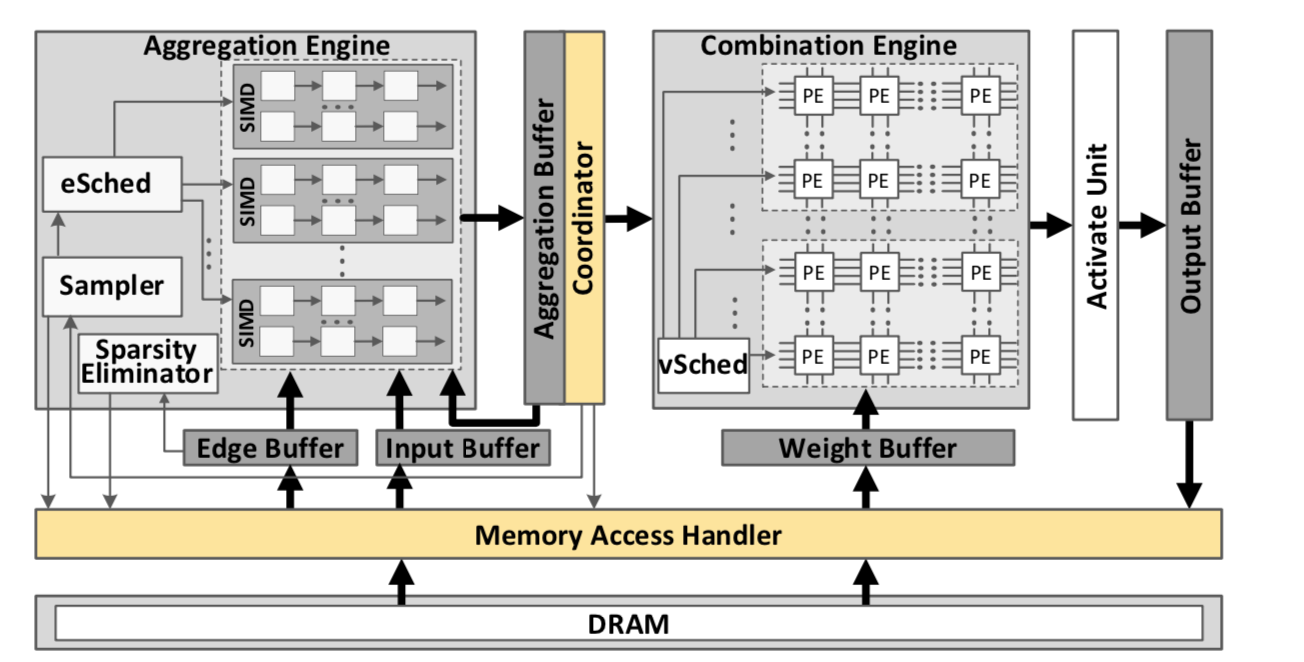
\includegraphics[width=\textwidth]{hygcn.png}
    \caption{加速器整体架构图}
\end{figure}

\subsection{聚集引擎}
聚合过程中主要考虑挖掘边级并行性。
为了支持采样操作,聚集引擎中引入了采样器,用于通过邻居的索引读取相应的邻边。
每个顶点有很多入边,通过边任务调度器eSched将边处理的任务分配到SIMD核上。
SIMD核内有两种工作模式,分别是顶点集中模式和顶点分散模式。
顶点集中模式将每个顶点的工作量分给一个SIMD核心,即定期处理一组顶点,但不同的顶点处理速度不全相同,可能导致负载不均衡。
顶点分散模式将每个顶点特征向量中各个维度分量的聚集过程分配给各个核,而不是将每个顶点的计算任务分配给各个核,如图3.2所示\footnote{图3.2引用自论文Hygcn: A GCN accelerator with hybrid architec­ture}。
如果一个顶点的任务不能占据所有核,则可以自由地将核分配给其他顶点的某个维度。
因此所有核都在工作而不会出现负载不均衡的情况,并且由于充分利用了顶点内部并行性,单个顶点的处理延迟小于多个顶点一起处理的平均延迟。
另外,每个顶点处理完成后,可供之后的组合引擎立即使用。

\begin{figure}[htb]
    \centering
    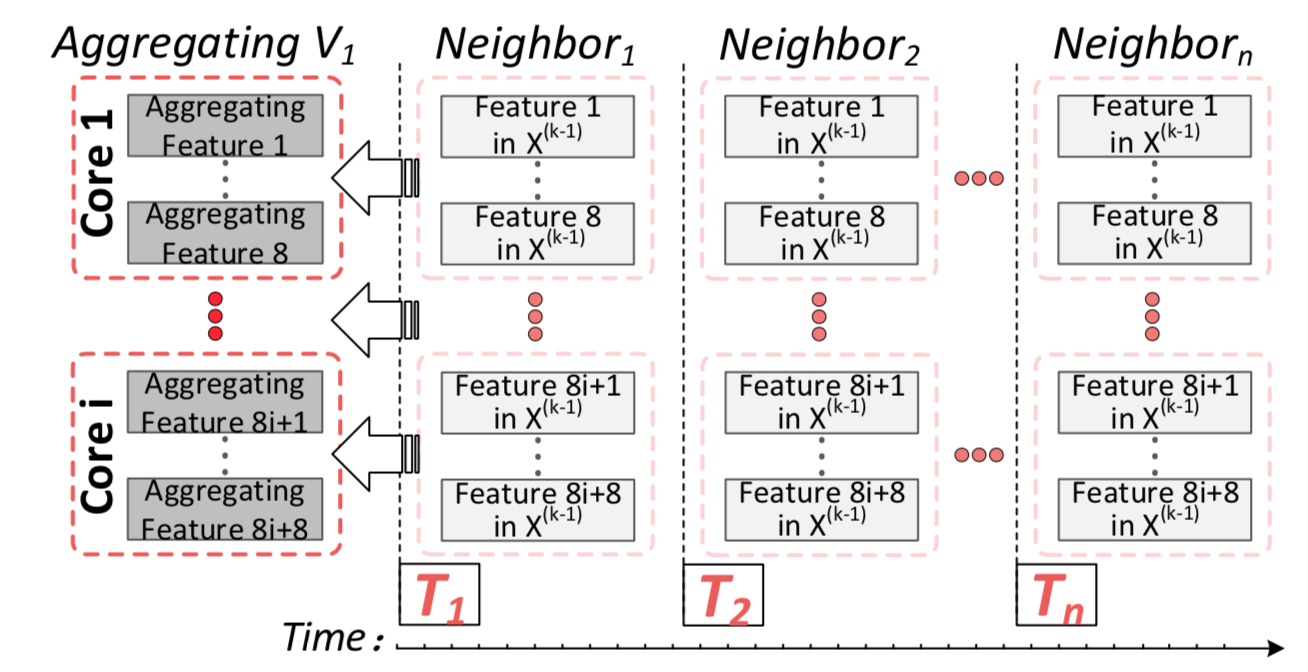
\includegraphics[width=\textwidth]{aggregation.png}
    \caption{顶点分散模式聚集}
\end{figure}

\subsection{组合引擎}
组合过程与传统神经网络前向传播的过程类似,为了提高处理并行性和数据重用性,组合引擎采用了脉动阵列设计,将一组脉动阵列拼在一起形成脉动模块。
主要任务是将来自聚集缓冲区和参数缓冲区的数据作为输入,执行矩阵运算,通过顶点调度器vSched分配计算任务。
矩阵运算的输出连接激活单元,根据不同类型取激活后生成新的顶点特征向量。

组合引擎有独立工作模式和合作工作模式,分别如图3.3(a)和(b)所示\footnote{图3.3引用自论文Hygcn: A GCN accelerator with hybrid architec­ture}。
\begin{itemize}
    \item 独立工作模式下脉动模块彼此独立工作,每个都处理一小组顶点的矩阵运算。每个模块的参数矩阵都可以直接从参数缓冲区获取,并在模块内重用。此模式的优点是,一旦一小组顶点的聚集过程结束,就可以立即进行这组顶点的组合过程而无须等待更多顶点,与聚集引擎的顶点分散处理模式能进行较好的协作。
    \item 合作工作模式下脉动模块可以进一步组装在一起以同时处理更多顶点。与独立工作模式不同的是,该模式在执行组合之前要等待一大组顶点的聚集过程结束。此模式的优势在于可以减少能量消耗。
\end{itemize}

\begin{figure}[htb]
    \centering
    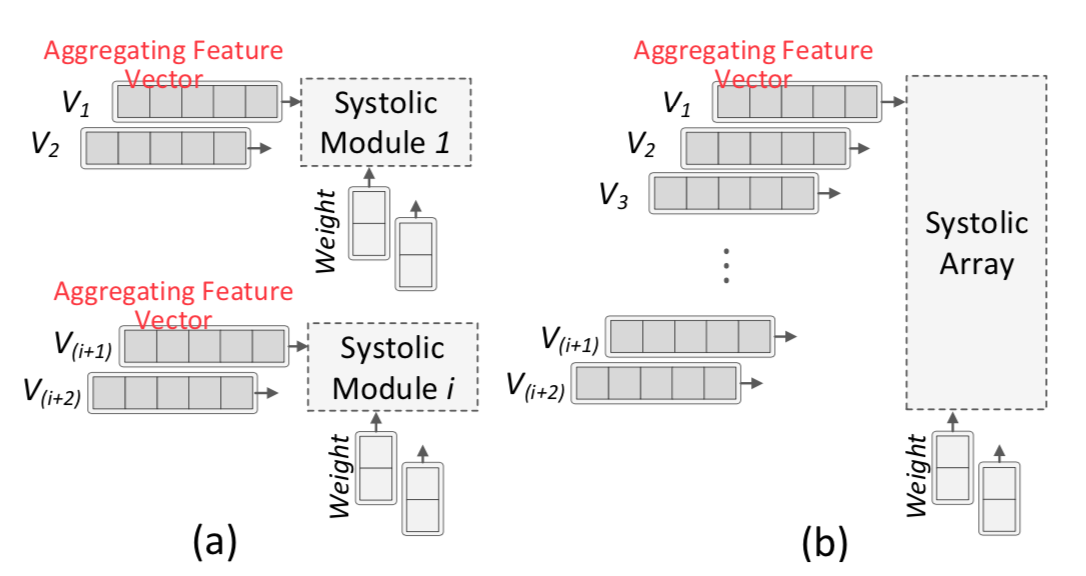
\includegraphics[width=\textwidth]{combination.png}
    \caption{两种工作模式:(a)独立工作模式;(b)合作工作模式}
\end{figure}

无论采用哪种模式,这种设计的组合引擎均有效提高了参数矩阵数据的重用率。

\subsection{协调器}
为了有效地融合聚集和组合的过程,使用聚集引擎和组合引擎之间的协调器来协调两个引擎对DRAM的访问。
由于实际运行时聚集阶段和组合阶段的相对运算量存在变化,难以确定两个引擎内存带宽的相对比值,故只使用一个片外存储器。
根据第一节整体架构中所述,总共有四个缓冲区用于访问片外存储器,存在大量并发访存的过程,如果依次处理这些访存请求,那么无规则的地址将大大降低缓冲区的利用率。
为了解决这一问题,预先定义访存优先级:边>输入特征>权重>输出特征,该顺序是处理顶点时的访存顺序。此举有助于利用空间局部性,因而可以显著提高访存效率。